\chapter{実験方法}
\section{概要}
\section{粘度計測}
粘度計測における計測機器の模式図を図に示す。ステージと回転する円錐回転子の間に存在する試料によって付加されるトルクを計測することで粘度の計測を行う。粘度のせん断速度依存性を確認することで生成した溶液の性質の確認を行った。なお、計測範囲の都合上、水道水では

\begin{figure}[htp]
    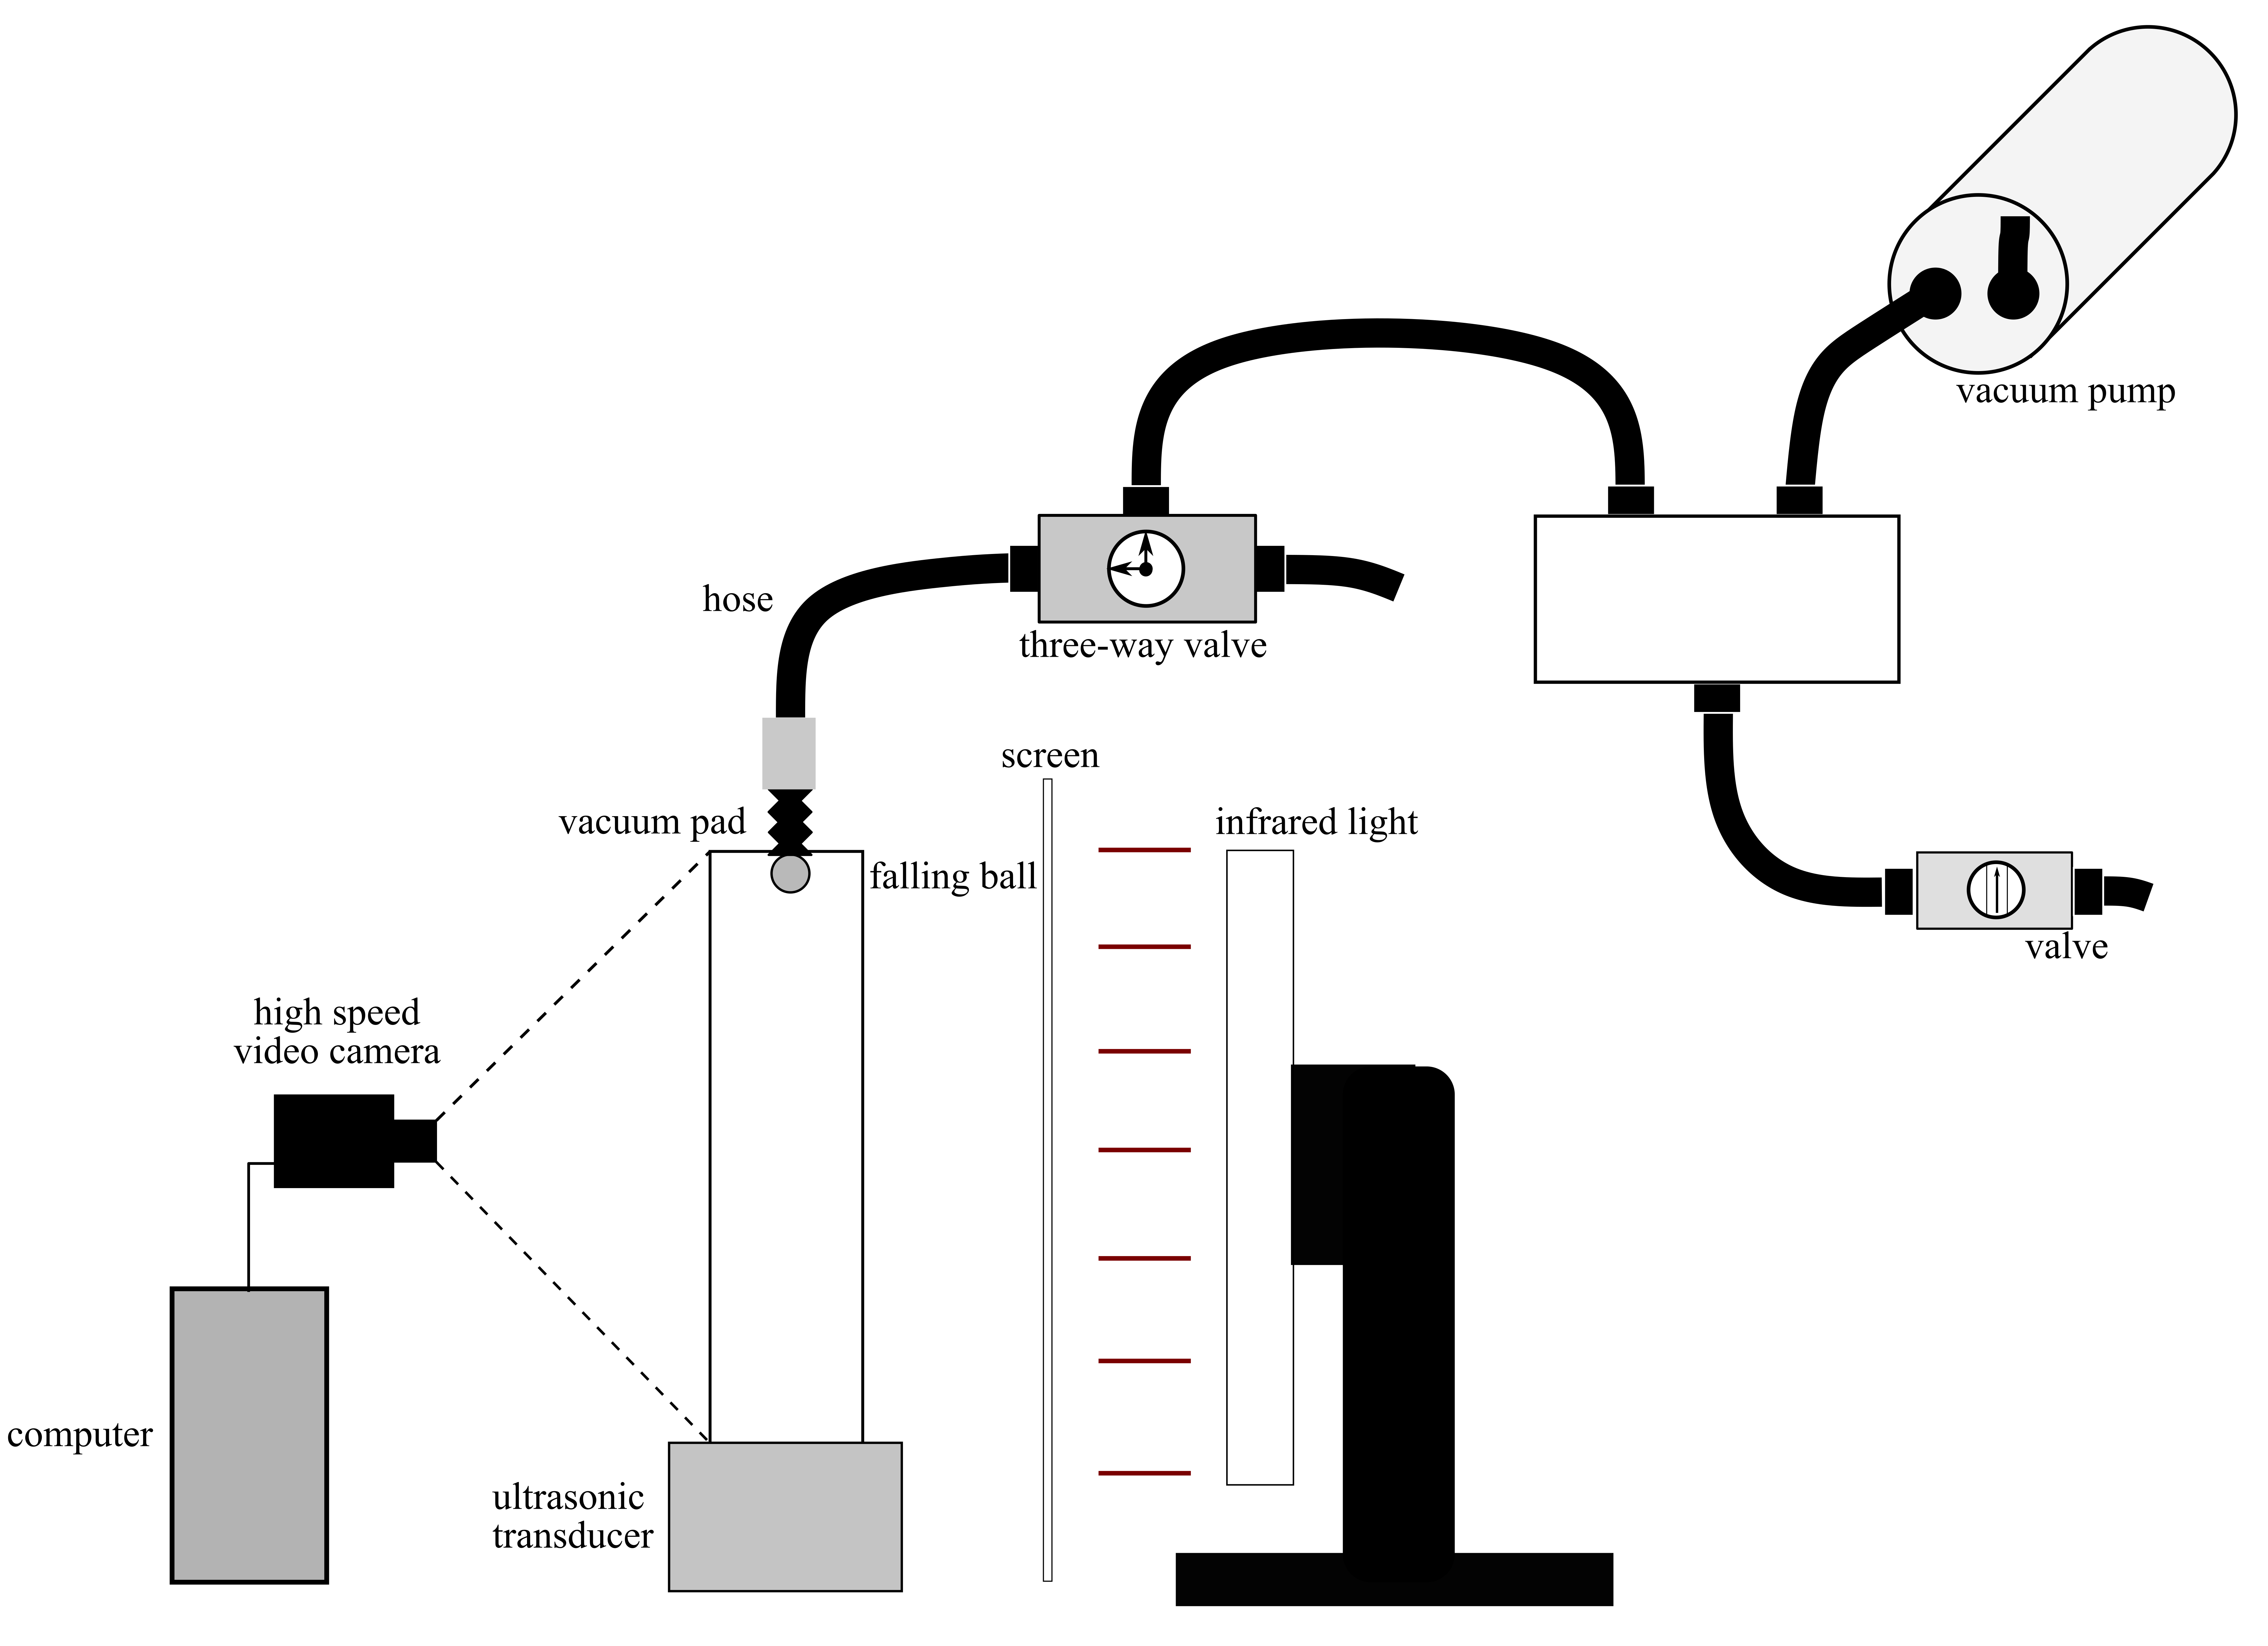
\includegraphics[clip,width=7.0cm]{2-Methods/device.png}
\end{figure}